\documentclass[../main.tex]{subfiles}

\begin{document}

\chapter{June $28^{th} / 2025$}
\label{ch:tufte-design}

\textbf{RECAP:}
\begin{itemize}
    \item Pathogenic (P): Sufficient evidence to be considered disease-causing
    \item Likely Pathogenic (LP): Evidence strongly suggests pathogenicity, but is not definitive
    \item Variant of Uncertain Significance (VUS): Insufficient or conflicting evidence to
classify as either pathogenic or benign
    \item Likely Benign (LB): Evidence strongly suggests a benign (non-disease-causing)
impact
    \item Benign (B): Sufficient evidence to be considered not disease-causing
\end{itemize}

\textit{Such framework is fundamentally probabilistic. 'Likely' categories $> 90\%$ certainty. Inherent probabilistic $must$ be captured by predictive model!}

\vspace{0.3cm}

Such guidelines have shown to reduce reclassification rates.

\hrulefill

\subsection{How Evidence Drives Reclassification?}

Reclassification rates ranges from $3.6\%$ to $58.6\%$ (really retarded range) underscoring the \textit{volatility} of initial classifications and importance of a continuous influx of new data.

Accumulation of information from multiple sources drives classification:
\begin{itemize}
    \item \textbf{Functional Studies} such as multiplex assays of variant effects (MAVEs) measure functional impact of variant on protein function (time consuming and resource intensive)
    \item \textbf{Computational / \textit{In Silico} Data} AlphaMissense provides novel in silico evidence for reclassification (analysis of evolutionary conservation and predicted structural impact)
    \item \textbf{Population Data} gnomAD provides frequency of variants in general population. e.g., variant common in healthy subjects is less likely to be pathogenic for a rare disease
    \item \textbf{Segregation Data} family studies / segregation studies to track whether x variant co-occurs with a disease across multiple family members
    \item \textbf{Literature and case reports} linking variants to phenotype
\end{itemize}

\subsection{VUS}

VUS imply a lack of compelling evidence to confidently place a variant under a category $\rightarrow$ Bottleneck in clinical genetics. A model that fails to predict a VUS-to-Pathogenic transition has made a more clinically significant error than one that misses an LP-to-P transition $\rightarrow$ A model's loss function could be customized to more \textbf{heavily penalize errors} optimizing model to align with clinical utility.

\section{Categorical Time-Series Problem}

The reclassification of variants can be seen as a \textbf{Time-ordered sequence of categorical labels}. e.g., Classification of variant $x$ at time $t$ is \textbf{dependent} on classification at $t-1$ $+$ cumulative evidence at $t$ $\rightarrow$ Temporal Dependency. Fundamental problem: Ground truth is \textit{non-stationary}. Whatever constitutes a pathogenic variant is refined over time, so statistical properties of data-generating process are \textit{changing}.

\vspace{0.2cm}

\textbf{Concept Drift:} Phenomenon where statistical relationships between input data and target variables change over time, usually in dynamic environments.
\textit{Patterns a machine learning model learned from historical data may no longer be valid as the real-world environment evolves}. So, how to solve such problem?

\begin{center}
    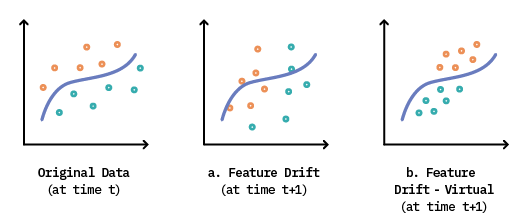
\includegraphics[width=12cm]{files/images/drift.png}    
\end{center}

\section{Framing a Predictive Task as Concept Drift}
Simple time-series forecasting models assume that underlying patterns in data are stable over time. Variant classification violates such assumption! since its intrinsic properties  and designed classification evolves as knowledge grows. A

A \textbf{stationary process} is one in which $\mu$ and $\sigma^2$ remain constant over time. Therefore, variant classification is an inherently non-stationary process. Concept drift $=$ non-stationary process but in supervised learning context $\rightarrow$ \textit{Change over time in the statistical relationship between input $X$ and target variable $Y$, $P(y|X)$}. Intrinsic features of a variant (e.g., genomic location, nucleotide change...) are static BUT interpretation of such features (concept of pathogenicity) evolves. So NOT the same as \textbf{Data Drift} where $P(X)$ changes.

\subsection{Drift Patterns}
\begin{itemize}
    \item \textbf{Abrupt Drift:} rapid and sudden change in data distribution. It could be triggered by a singular, high impact event, e.g., publication of 2015 ACMG/AMP guidelines
    \item \textbf{Gradual Shift:} Slow, incremental change over a long period. \textit{Likely observed in variant classification}. Evidence accumulates over time, slowly shifting balance of evidence for or against pathogenicity
    \item \textbf{Recurring Drift:} Cyclical changes. Less common in variant reclassification.
\end{itemize}

The timestamp of reclassification serves as proxy for state of scientific knowledge and classification standards in place at $t$. Thus, time-related features (e.g., time elapsed since last classification, binary indicators for guideline changes) MUST be incorporated into model's input.

A \textbf{Stream Learning} framework \textit{MUST} be so it can adapt and evolve as new data becomes available.

\subsection{Strategies for Model Updating}
\begin{itemize}
    \item \textbf{Periodic Retraining} Retained from scratch at regular intervals (every x months) using data up to $t$
    \item \textbf{Triggered Retraining} COntinuously monitor model's performance on new incoming data. An algorithm such as \textbf{Drift Detection Method (DDM)} or \textbf{LSTM-based detector (LSTMDD)} is used to identify a statistically significant drop in performance. When drift is detected $\rightarrow$ Trigger MODEL RETRAINING. NO unnecessary monthly/annual updates while $'concept'$ $=$ $stable$
    \end{itemize}

    THEREFORE, model must be able to learn historical patterns AND patterns of \textit{how those patterns themselves change!}. An LSTM will capture temporal dependencies BUT it MUST be embedded within a larger online framework that manages its lifecycle of training, evaluation, and updating.

\section{Temporal Long Short-Term Memory (LSTM)}

Before LSTM learns from temporal sequences of variant reclassification:  
\begin{enumerate}
    \item encode categorical classification labels into numerical format
    \item transform continuous-time series data into discrete input-output windows suitable for supervised learning
\end{enumerate}

\section{Entity Embedding}

    From NLP (e.g., Word2Vec), it maps each category to a dense, low dimensional vector of continuous values (for each category within a categorical feature). Vectors are not predefined but learned by NN. An embedding layer is added to the model which learns to place categories that are semantically similar closer to each other in the multi-dimensional embedding space $\rightarrow$ Model can autonomously discover that LP and P should have similar vector representations, while B should be distant from them. Entity embeddings thus provide dense and \textbf{contextually} aware representation. Also good for sparce or complex categorical data. 

\vspace{0.2cm}

\textbf{Embedding Layer}: Core component of entity embeddings. It is pretty much a lookup table which is represented as a weight matrix.

\subsection{Embedding Matrix}

Let $C$ be a categorical feature with a vocabulary of size $V$. This means the feature has $V$ unique categories (e.g., if the feature is "Gene Symbol", $V$ would be the total number of unique gene symbols in the dataset).

Let $D$ be the desired dimensionality of embedding vectors. This is a hyperparameter (e.g., $D=10$, $D=50$)

The embedding layer maintains a single weight matrix, \textbf{embedding matrix}, $E$.

\begin{equation}
    E \in \mathbb{R}^{V \times D}
\end{equation}

Each row $e_i$ of matrix $E$ is the $D$-dimensional embedding vector for the $i$-th category in the vocabulary.

\[
E =
  \begin{bmatrix}
    --- & e_1 & --- \\
    --- & e_2 & --- \\
    \vdots & \vdots & \vdots \\
    --- & e_V & ---
  \end{bmatrix}
=
  \begin{bmatrix}
    e_{11} & e_{12} & \dots & e_{1D} \\
    e_{21} & e_{22} & \dots & e_{2D} \\
    \vdots & \vdots & \ddots & \vdots \\
    e_{V1} & e_{V2} & \dots & e_{VD}
  \end{bmatrix}
\]

Initially, matrix is filled with small random values. The goal of training is to learn optimal values for all entries in matrix

\subsection{Embedding Lookup Operation}

The input to an embedding layer is typically an integer representing a specific category (e.g., category "Gene Symbol: BRCA1" might be mapped to integer index 15). The layer performs a simple \textbf{lookup operation} to retrieve the corresponding embedding vector.

Lookup can be represented as a matrix multiplication with a one-hot encoded vector. Let the input category be represented by integer $k$, where $1 \le k \le V$. Then represent this input as a one-hot vector $c_k$ of size $V$, where $k$-th element is 1 and all other elements are 0.

\begin{equation}
    c_k = [0, 0, \dots, 1, \dots, 0]^T
\end{equation}

The output of the embedding layer, which is the embedding vector for category $k$, is then given by:

\begin{equation}
    v_k = E^T \cdot c_k
\end{equation}

This matrix multiplication selects the $k$-th column of $E^T$, which is the $k$-th row of $E$. NNs don't go through all this BS with matrices, this is just for simplification.

\subsection{Learning Embeddings}

Values of embedding matrix $E$ are learned (backpropagation). The network is trained on a supervised task (e.g., predicting variant pathogenicity).

\subsection{Objective Function (Loss Function)}

Let the neural network be denoted by a function $f$, which takes the learned embeddings and other features as input to make a prediction $\hat{y}$. The network learns by minimizing a loss $L(\hat{y}, y)$

For a classification task, a common loss function is the **Binary Cross-Entropy Loss**:

\begin{equation}
    L(\hat{y}, y) = - \frac{1}{N} \sum_{i=1}^{N} \left[ y_i \log(\hat{y}_i) + (1 - y_i) \log(1 - \hat{y}_i) \right]
\end{equation}

$\hat{y}_i = f(v_{k_i}, \dots)$ is output for $i$-th training, which includes embedding vector $v_{k_i}$ for category $k$

\subsection{Updating Embedding Matrix (Backpropagation)}

Use of optimization algorithm  (e.g., Stochastic Gradient Descent (SGD), Adam) to update all weightsn and embedding matrix $E$.

For a single training example, the gradient of the loss $L$ with respect to the embedding matrix $E$ is calculated. An important property of the embedding lookup operation is that the gradient is \textbf{sparse}. For an input category $k$, only $k$-th row of the embedding matrix, $e_k$, contributed to the final output. Therefore, the gradient will be non-zero only for that specific row.

\begin{equation}
    \frac{\partial L}{\partial e_j} = 0 \quad \text{for all } j \neq k
\end{equation}

The non-zero gradient is for the vector $e_k$ that was used in the forward pass:

\begin{equation}
    \frac{\partial L}{\partial e_k} = \frac{\partial L}{\partial \hat{y}} \frac{\partial \hat{y}}{\partial e_k}
\end{equation}

Update e.g., standard SGD with learning rate $\eta$:

\begin{equation}
    e_k^{(\text{new})} = e_k^{(\text{old})} - \eta \frac{\partial L}{\partial e_k}
\end{equation}

Over many training iterations, each row of the embedding matrix is adjusted based on how it contributes to the overall prediction error for the categories it represents. This process causes vectors for categories that appear in similar contexts (with respect to the prediction target) to be pushed closer together in the embedding space.

\vspace{0.3cm}

Determining the optimal window size $`n past`$ is a critical hyperparameter tuning task.
\begin{itemize}
    \item Most variant classifications occur within $\approx2$ years of initial classification. If data is recorded quarterly then window size of $8$ ($2$ years) is a logical initial value for test
    \item Treat window size as hyperparameter and evaluate performance \textit{dedicated} validation set
\end{itemize}

\section{Validation for Temporal Data}
For data with temporal dependencies, such as variant reclassification histories standard validation techniques are inappropriate guaranteed to produce misleading and  way too optimistic results

Let a time-series dataset be an ordered sequence of observations $D = \{ (x_1, y_1), (x_2, y_2), \dots, (x_T, y_T) \}$, where $T$ is total number of observations.

The process creates a series of $k$ splits, where each split consists of a training set ($D_{\text{train}}^{(i)}$) and a validation set ($D_{\text{val}}^{(i)}$).

\subsection*{Splitting}

Let $n_0$ be the size of the initial training set, and let $h$ be the size of the validation set (the forecast horizon). The splits are generated iteratively.

For each split $i = 1, 2, \dots, k$:

\begin{itemize}
    \item \textbf{Training Set ($D_{\text{train}}^{(i)}$):} The training set includes all data from the beginning up to a certain point in time. It expands with each iteration.
    \begin{equation}
        D_{\text{train}}^{(i)} = \{ (x_t, y_t) \mid t = 1, \dots, n_0 + (i-1)h \}
    \end{equation}

    \item \textbf{Validation Set ($D_{\text{val}}^{(i)}$):} The validation set consists of the next $h$ observations immediately following the training set.
    \begin{equation}
        D_{\text{val}}^{(i)} = \{ (x_t, y_t) \mid t = (n_0 + (i-1)h) + 1, \dots, n_0 + ih \}
    \end{equation}
\end{itemize}

The constraint $n_0 + k \cdot h \le T$ must be satisfied. This ensures that the validation set for the final split does not exceed the total number of observations.

\subsection*{Model Evaluation}

A model, $M$, is trained on each training set $D_{\text{train}}^{(i)}$ to produce a trained model $M_i$. The performance of each model $M_i$ is then evaluated on its corresponding validation set $D_{\text{val}}^{(i)}$ using a chosen error metric, $\mathcal{L}$ (e.g., Mean Squared Error, Mean Absolute Error). Let this error be $\text{Err}_i$.

\begin{equation}
    \text{Err}_i = \mathcal{L}(M_i, D_{\text{val}}^{(i)})
\end{equation}

The overall performance estimate for the model $M$ is the average of the errors across all $k$ splits.

\begin{equation}
    \text{CV}_{\text{Error}} = \frac{1}{k} \sum_{i=1}^{k} \text{Err}_i
\end{equation}

This procedure ensures that at no point is the model trained on data that occurred chronologically after the data it is being asked to predict, thus preserving the temporal integrity of the dataset.

\vspace{0.3cm}

\textbf{Nested Cross-Validation is pprobably better than the above strategy!}

\section{Probabilistic Forecasting}
\textbf{Goal} is to predict single most likely next classification for x variant. Model's uncertainty is paramount. e.g., A prediction of "Pathogenic" with $51\%$ confidence carries a vastly different clinical implication than a prediction with $99\%$ confidence. Therefore, the task should be framed as \textbf{probabilistic classification} where model outputs a full probability distribution over all possible future classes

Architecture must be designed as follows:
\begin{itemize}
    \item \textbf{Output Layer:} Final Layer of LSTM should be a \textit{Dense (fully connected)} layer
    \item \textbf{Activation Function:} Dense layer must use \textbf{softmax activation function}. in: logits, out: probability vector
    \item \textbf{Number Neurons:} Must equal to number of classes in classification system (B, LB, VUS, LP, P). 

    e.g., Input sequence = vector [0.05, 0.10, 0.10,
0.60, 0.15], representing a $5\%$ chance of being Benign, $10\%$ Likely Benign, $10\%$ VUS, $60\%$ Likely Pathogenic, and $15\%$ Pathogenic

\begin{itemize}
    \item \textbf{Attention Mechanism}: Attention layer to allow LSTM to dynamically assign different weights of important to different time steps in the input sequence when making a prediction.
    \item \textbf{Stacked LSTM:} Multiple layers can be stacked on top of each other to allow model to learn a hierarchical representation of the temporal data. e.g., first layer may learn simple short-term patterns, while deeper
layers could combine these to learn more complex, long-term abstract patterns in the reclassification sequence
\end{itemize}

\end{itemize}

\end{document}